\documentclass[10pt]{beamer}

%\usetheme[progressbar=frametitle]{metropolis}
\usepackage{appendixnumberbeamer}
\usepackage{attrib}
\usepackage{booktabs}
\usepackage[scale=2]{ccicons}

\usepackage{xspace}
%\newcommand{\themename}{\textbf{\textsc{metropolis}}\xspace}
%%%%%%%%%%%%%%%%%%%%%%%%
\usepackage{minted}

\graphicspath{images/}

%%%%%%%%%%%%%%%%%%%%%%%%
\title{datetime}
\subtitle{A Tale of Pythonic Woe}
% \date{\today}
\date{23 August 2017}
\author{Dave Voutila}
\institute{Sisu Integrated Services, LLC}
% \titlegraphic{\hfill\includegraphics[height=1.5cm]{logo.pdf}}

\begin{document}

\maketitle

\begin{frame}{Table of contents}
  \setbeamertemplate{section in toc}[sections numbered]
  \tableofcontents[hideallsubsections]
\end{frame}

\begin{frame}[fragile]{Backstory}
\begin{itemize}
\item Contributor to \textbf{Flask-Ask}, a Python Amazon Alexa framework.
\item Jumped on \textit{Issue 152: Flask Ask doesn't parse time stamp from Alexa properly...}
\item Things when downhill from there...
\end{itemize}

\end{frame}

\begin{frame}{The Problem}
\begin{center}
	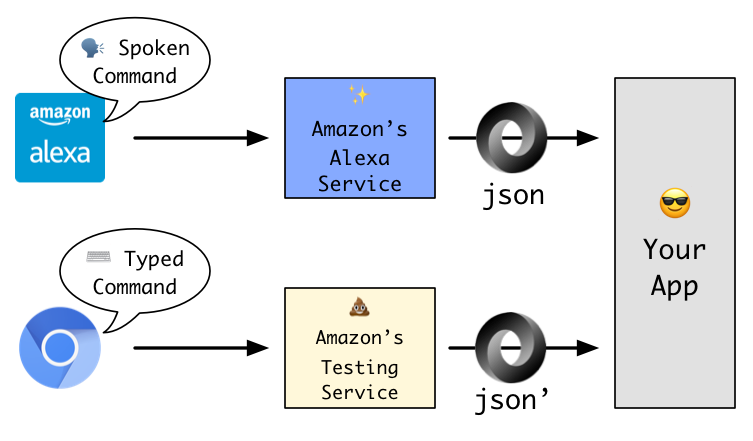
\includegraphics[width=9cm]{./images/alexa-flow.png}
	\begin{alertblock}{Attention}
		json != json'
	\end{alertblock}
\end{center}
\end{frame}

\begin{frame}{A Tale of Two Timestamps}
\begin{columns}
	\begin{column}{0.5 \textwidth}
		\begin{itemize}
			\item Let's see what Amazon says (\textbf{emphasis} mine):
		\end{itemize}
	\end{column}
	\begin{column}{0.5 \textwidth}
		\begin{quote}
			The timestamp is provided as an \textbf{ISO 8601 formatted string} (for example, 2015-05-13T12:34:56Z). Your code needs to parse the string into a date object, then verify that it is within the tolerance your web service allows...
\\\
		--- \href{https://developer.amazon.com/public/solutions/alexa/alexa-skills-kit/docs/developing-an-alexa-skill-as-a-web-service\#timestamp}{\textbf{Amazon's} Checking the Timestamp of a Request}
		\end{quote}
	\end{column}
\end{columns}
\end{frame}

\begin{frame}{Good vs. Evil}
\begin{columns}
	\begin{column}{0.5 \textwidth}
		\inputminted[fontsize=\small,frame=single,framesep=2mm,linenos=true,breaklines]{javascript}{src/good.json}
	\end{column}
	\begin{column}{0.5 \textwidth}
		\inputminted[fontsize=\small,frame=single,framesep=2mm,linenos=true,breaklines]{javascript}{src/bad.json}
	\end{column}
\end{columns}
\end{frame}

\renewcommand{\arraystretch}{1.5}
\begin{frame}{Python and Time}
\begin{center}
\begin{tabular}{ c c c }
Language & Example & Precision \\
\hline
Go & \mintinline{go}{time.Time} & nanoseconds \\
Java & \mintinline{java}{java.lang.System.getNanos()} & nanoseconds \\
C\# & \mintinline{csharp}{DateTime.Ticks} & \(\frac{1}{10}\) microseconds \\
Javascript & \mintinline{javascript}{Date.now()} & milliseconds \\
Python & \mintinline{python}{time.time()} & microseconds
\end{tabular}
\end{center}
\end{frame}

\begin{frame}{Python Time Canon}
Just what is canonical in Python?

\end{frame}
\end{document}

